\documentclass[12pt,a4paper]{article}
\usepackage[utf8]{vietnam}
\usepackage{amsmath,amssymb}
\usepackage{tabularx}
\usepackage{tikz}
\usetikzlibrary{calc,angles,quotes,arrows.meta,patterns}
\usepackage{xcolor}
\usepackage{enumitem}
\usepackage{fancyhdr}
\usepackage[top=1.2cm, bottom=1.2cm, left=1.5cm, right=1.5cm]{geometry}
\usepackage[loigiai]{ex_test}
\SAOPTN{widthSA=2.6,heightSA=0.62}

\setlength{\headheight}{15pt}
\setlength{\parskip}{0pt}

\pagestyle{fancy}
\fancyhf{}
\rhead{\textit{Môn Toán 6 -- Hướng dẫn giải Đề số 1}}
\lhead{\textit{Bộ đề ôn tập Giữa học kì I}}
\cfoot{\thepage}

\begin{document}

\begin{center}
  \textbf{\Large HƯỚNG DẪN GIẢI CHI TIẾT VÀ BẢNG ĐÁP ÁN}\\
  \textbf{\large ĐỀ ÔN TẬP GIỮA HỌC KỲ I -- ĐỀ SỐ 1}\\
  \textit{Môn: Toán 6 -- Năm học 2026 -- 2027}
\end{center}
\vspace{2mm}

% --- BẢNG ĐÁP ÁN TRẮC NGHIỆM TÓM TẮT ---
\noindent\textbf{\large A. BẢNG ĐÁP ÁN TRẮC NGHIỆM TỔNG HỢP}
\vspace{1.5mm}

\noindent\textbf{1. Phần I (Mỗi câu trả lời đúng được 0,25 điểm):}
\begin{center}
\begin{tabular}{|c|c|c|c|c|c|c|c|c|c|c|c|c|}
\hline
\textbf{Câu} & \textbf{1} & \textbf{2} & \textbf{3} & \textbf{4} & \textbf{5} & \textbf{6} & \textbf{7} & \textbf{8} & \textbf{9} & \textbf{10} & \textbf{11} & \textbf{12} \\
\hline
\textbf{Đ/A} & \textbf{C} & \textbf{A} & \textbf{C} & \textbf{B} & \textbf{D} & \textbf{D} & \textbf{B} & \textbf{D} & \textbf{B} & \textbf{B} & \textbf{A} & \textbf{D} \\
\hline
\end{tabular}
\end{center}
\vspace{1mm}

\noindent\textbf{2. Phần II (Đúng/Sai):}
\begin{center}
\begin{tabular}{|c|c|c|c|c||c|c|c|c|c|}
\hline
\textbf{Câu 1} & \textbf{a)} & \textbf{b)} & \textbf{c)} & \textbf{d)} & \textbf{Câu 2} & \textbf{a)} & \textbf{b)} & \textbf{c)} & \textbf{d)} \\
\hline
\textbf{Đ/S} & \textbf{Đ} & \textbf{Đ} & \textbf{S} & \textbf{S} & \textbf{Đ/S} & \textbf{Đ} & \textbf{Đ} & \textbf{Đ} & \textbf{Đ} \\
\hline
\end{tabular}
\end{center}
\vspace{1mm}

\noindent\textbf{3. Phần III (Mỗi câu trả lời đúng được 1,0 điểm):}
\begin{center}
\begin{tabular}{|c|c|c|}
\hline
\textbf{Câu} & \textbf{Câu 1} & \textbf{Câu 2} \\
\hline
\textbf{Đáp án} & \textbf{1} & \textbf{6} \\
\hline
\end{tabular}
\end{center}
\vspace{3mm}

% --- LỜI GIẢI CHI TIẾT ---
\noindent\textbf{\large B. HƯỚNG DẪN GIẢI CHI TIẾT TỪNG CÂU}
\vspace{2mm}

\noindent\textbf{\large PHẦN I. CÂU TRẮC NGHIỆM NHIỀU PHƯƠNG ÁN LỰA CHỌN}
\vspace{1mm}
\begin{ex}
Tập hợp nào dưới đây là tập hợp số tự nhiên?
\choice
{$\mathbb{N} = \{1; 2; 3; \dots\}$}
{$\mathbb{N} = \{0; 1; 2; 3; \dots; 100\}$}
{\True $\mathbb{N} = \{0; 1; 2; 3; \dots\}$}
{$\mathbb{N} = \{0; 2; 4; 6; \dots\}$}
\loigiai{
Tập hợp các số tự nhiên được kí hiệu là $\mathbb{N}$, gồm các số $0, 1, 2, 3, \dots$ kéo dài vô hạn. Do đó $\mathbb{N} = \{0; 1; 2; 3; \dots\}$.
}
\end{ex}

\begin{ex}
Với $a, m, n$ là các số tự nhiên, khẳng định nào sau đây là đúng?
\choice
{\True $a^m : a^n = a^{m-n}$ ($a \neq 0, m \geq n$)}
{$a^m : a^n = a^{m+n}$ ($a \neq 0$)}
{$a^m \cdot a^n = a^{m:n}$ ($a \neq 0$)}
{$a^m : a^n = m - n$ ($a \neq 0$)}
\loigiai{
Theo quy tắc chia hai lũy thừa cùng cơ số: Khi chia hai lũy thừa cùng cơ số (khác 0), ta giữ nguyên cơ số và trừ các số mũ: $a^m : a^n = a^{m-n}$ ($a \neq 0, m \geq n$).
}
\end{ex}

\begin{ex}
Thứ tự thực hiện phép tính nào sau đây là đúng đối với biểu thức không có dấu ngoặc?
\choice
{Nhân và chia $\to$ Lũy thừa $\to$ Cộng và trừ}
{Cộng và trừ $\to$ Nhân và chia $\to$ Lũy thừa}
{\True Lũy thừa $\to$ Nhân và chia $\to$ Cộng và trừ}
{Cộng và trừ $\to$ Lũy thừa $\to$ Nhân và chia}
\loigiai{
Đối với biểu thức không có dấu ngoặc, thứ tự thực hiện phép tính chuẩn là: Lũy thừa $\to$ Nhân và chia $\to$ Cộng và trừ.
}
\end{ex}

\begin{ex}
Hình vuông $ABCD$ có cạnh $AB = 3\text{ cm}$. Diện tích của hình vuông đó là:
\choice
{$3\text{ cm}^2$}
{\True $9\text{ cm}^2$}
{$12\text{ cm}^2$}
{$81\text{ cm}^2$}
\loigiai{
Diện tích hình vuông $ABCD$ là: $S = a^2 = 3^2 = 9\text{ cm}^2$.
}
\end{ex}

\begin{ex}
Số $19$ trong hệ La Mã được viết là:
\choice
{IX}
{IXX}
{XXI}
{\True XIX}
\loigiai{
Ta phân tích $19 = 10 + 9$. Trong chữ số La Mã: $10$ là $\mathrm{X}$ và $9$ là $\mathrm{IX}$. Do đó $19$ được viết là $\mathrm{XIX}$.
}
\end{ex}

\begin{ex}
Trong các phân số sau, phân số nào là phân số tối giản?
\choice
{$\dfrac{26}{39}$}
{$\dfrac{15}{12}$}
{$\dfrac{27}{42}$}
{\True $\dfrac{3}{16}$}
\loigiai{
Ta có: $\dfrac{26}{39} = \dfrac{2}{3}$ (chia cho 13); $\dfrac{15}{12} = \dfrac{5}{4}$ (chia cho 3); $\dfrac{27}{42} = \dfrac{9}{14}$ (chia cho 3). Phân số $\dfrac{3}{16}$ có $\text{ƯCLN}(3, 16) = 1$ nên là phân số tối giản.
}
\end{ex}

\begin{ex}
Tập hợp các chữ cái trong cụm từ “PHONG NHA” là:
\choice
{$\{P; H; O; N; G; N; H; A\}$}
{\True $\{P; H; O; N; G; A\}$}
{$\{H; O; N; G; P; A\}$}
{$\{N; A; P; O; G\}$}
\loigiai{
Khi viết tập hợp các chữ cái của một từ, mỗi chữ cái chỉ được liệt kê một lần. Các chữ cái trong từ “PHONG NHA” gồm $P, H, O, N, G, A$. Do đó tập hợp là $\{P; H; O; N; G; A\}$.
}
\end{ex}

\begin{ex}
Trong các số sau, số nào là bội của $7$?
\choice
{$15$}
{$20$}
{$25$}
{\True $35$}
\loigiai{
Ta có $35 : 7 = 5$ (chia hết) nên $35$ là bội của $7$.
}
\end{ex}

\begin{ex}
Thực hiện phép tính $3^2 + 3^3$ được kết quả là:
\choice
{$45$}
{\True $36$}
{$432$}
{$423$}
\loigiai{
Ta có: $3^2 + 3^3 = 9 + 27 = 36$.
}
\end{ex}

\begin{ex}
\immini{
Từ hình bên có bao nhiêu hình vuông?
\choice
{$4$ hình vuông}
{\True $5$ hình vuông}
{$6$ hình vuông}
{$8$ hình vuông}
}{
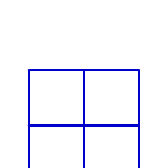
\begin{tikzpicture}[scale=0.7, baseline=(current bounding box.center), line cap=round, line join=round]
  \draw[step=1cm, thick, blue!80!black] (0,0) grid (2,2);
\end{tikzpicture}
}
\loigiai{
Có $4$ hình vuông nhỏ kích thước $1 \times 1$ và $1$ hình vuông lớn kích thước $2 \times 2$. Tổng cộng có $4 + 1 = 5$ hình vuông.
}
\end{ex}

\begin{ex}
Tập hợp tất cả các ước của số $20$ là:
\choice
{\True $\text{Ư}(20) = \{1; 2; 4; 5; 10; 20\}$}
{$\text{Ư}(20) = \{0; 1; 2; 4; 5; 10\}$}
{$\text{Ư}(20) = \{1; 2; 5; 10\}$}
{$\text{Ư}(20) = \{1; 2; 10; 20\}$}
\loigiai{
Lấy $20$ chia lần lượt cho các số từ $1$ đến $20$, các phép chia hết cho ta tập ước: $\text{Ư}(20) = \{1; 2; 4; 5; 10; 20\}$.
}
\end{ex}

\begin{ex}
Ghép $6$ tam giác đều có độ dài cạnh $3\text{ cm}$ thành một lục giác đều. Khi đó độ dài đường chéo chính của lục giác đều là:
\choice
{$9\text{ cm}$}
{$3\text{ cm}$}
{$12\text{ cm}$}
{\True $6\text{ cm}$}
\loigiai{
Lục giác đều gồm 6 tam giác đều ghép lại chung một đỉnh tâm. Đường chéo chính của lục giác đều đi qua tâm và bằng tổng độ dài 2 cạnh của tam giác đều: $3 + 3 = 6\text{ cm}$.
}
\end{ex}


\setcounter{ex}{0}
\noindent\textbf{\large PHẦN II. CÂU TRẮC NGHIỆM ĐÚNG SAI}
\vspace{1mm}
\begin{ex}
Cho $N$ là tập hợp các số tự nhiên chẵn nhỏ hơn $10$. Các khẳng định sau đây đúng hay sai?
\choiceTF
{\True Tập hợp $N$ được viết theo cách liệt kê các phần tử là $N = \{0; 2; 4; 6; 8\}$}
{\True Số phần tử của tập hợp $N$ là $5$ phần tử}
{Số $10$ thuộc tập hợp $N$ (kí hiệu $10 \in N$)}
{Tập hợp $N$ có thể được viết bằng cách chỉ ra tính chất đặc trưng là $N = \{x \in \mathbb{N} \mid x \text{ là số chẵn}\}$}
\loigiai{
\begin{itemize}[leftmargin=0.6cm, itemsep=1pt]
\item \textbf{a)} \textbf{Đúng}. Các số tự nhiên chẵn nhỏ hơn 10 là 0, 2, 4, 6, 8. Khẳng định đúng.
\item \textbf{b)} \textbf{Đúng}. Tập hợp $N$ gồm 5 phần tử $\{0, 2, 4, 6, 8\}$. Khẳng định đúng.
\item \textbf{c)} \textbf{Sai}. Tập hợp $N$ chỉ gồm các số chẵn nhỏ hơn 10 nên 10 không thuộc $N$ ($10 \notin N$). Khẳng định sai.
\item \textbf{d)} \textbf{Sai}. Cách viết này biểu diễn toàn bộ các số tự nhiên chẵn vô hạn, thiếu điều kiện giới hạn $x < 10$. Khẳng định sai.
\end{itemize}
}
\end{ex}

\begin{ex}
Cho hình chữ nhật $ABCD$ có độ dài cạnh $AB = 5\text{ cm}$ và $BC = 2\text{ cm}$. Các khẳng định sau đây đúng hay sai?
\choiceTF
{\True Độ dài cạnh $CD = 5\text{ cm}$ và độ dài cạnh $AD = 2\text{ cm}$}
{\True Chu vi của hình chữ nhật $ABCD$ bằng $14\text{ cm}$}
{\True Diện tích của hình chữ nhật $ABCD$ bằng $10\text{ cm}^2$}
{\True Hình chữ nhật $ABCD$ có $2$ trục đối xứng}
\loigiai{
\begin{itemize}[leftmargin=0.6cm, itemsep=1pt]
\item \textbf{a)} \textbf{Đúng}. Hình chữ nhật có các cặp cạnh đối diện bằng nhau: $CD = AB = 5\text{ cm}$, $AD = BC = 2\text{ cm}$. Khẳng định đúng.
\item \textbf{b)} \textbf{Đúng}. Chu vi hình chữ nhật là: $C = (AB + BC) \times 2 = (5 + 2) \times 2 = 14\text{ cm}$. Khẳng định đúng.
\item \textbf{c)} \textbf{Đúng}. Diện tích hình chữ nhật là: $S = AB \times BC = 5 \times 2 = 10\text{ cm}^2$. Khẳng định đúng.
\item \textbf{d)} \textbf{Đúng}. Hình chữ nhật có 2 trục đối xứng là hai đường trung trực của hai cặp cạnh đối diện. Khẳng định đúng.
\end{itemize}
}
\end{ex}


\setcounter{ex}{0}
\noindent\textbf{\large PHẦN III. CÂU HỎI TRẢ LỜI NGẮN}
\vspace{1mm}
\begin{ex}
Số liền trước của số nguyên tố nhỏ nhất là số mấy? \shortans{$1$}
\loigiai{
Số nguyên tố nhỏ nhất là số $2$. Số tự nhiên liền trước của số $2$ là số $1$.
}
\end{ex}

\begin{ex}
Mẹ Minh mua một túi gạo $15\text{ kg}$ loại $20\,000$ đồng mỗi $1\text{ kg}$. Hỏi mẹ Minh phải đưa cô bán hàng bao nhiêu tờ tiền loại $50\,000$ đồng để vừa đủ thanh toán tiền mua gạo trên? \shortans{$6$}
\loigiai{
Tổng số tiền mua gạo là: $15 \times 20\,000 = 300\,000$ đồng. Số tờ tiền loại $50\,000$ đồng cần trả là: $300\,000 : 50\,000 = 6$ (tờ).
}
\end{ex}


\setcounter{ex}{0}
\noindent\textbf{\large PHẦN IV. TỰ LUẬN (3,0 ĐIỂM - CÓ BAREM ĐIỂM CHI TIẾT)}
\vspace{1mm}
\begin{ex} (1.0 điểm)
Thực hiện phép tính (tính hợp lí nếu có thể):
\begin{enumerate}[label=\textbf{\alph*)}, leftmargin=0.8cm, itemsep=2pt]
\item $36 + 75 + 64 + 25 + 99$
\item $2024^0 + 3 \cdot [5^2 \cdot 10 - (23 - 13)^2]$
\item $4^2 \cdot 65 + 35 \cdot 4^2 - 1500$
\end{enumerate}
\loigiai{
\begin{itemize}[leftmargin=0.5cm, itemsep=3pt]
\item \textbf{a)} $36 + 75 + 64 + 25 + 99 = (36 + 64) + (75 + 25) + 99 = 100 + 100 + 99 = 299$. \hfill \textbf{[0.25đ]}
\item \textbf{b)} Ta có:\
$2024^0 + 3 \cdot [5^2 \cdot 10 - (23 - 13)^2] = 1 + 3 \cdot [25 \cdot 10 - 10^2] = 1 + 3 \cdot [250 - 100] = 1 + 3 \cdot 150 = 1 + 450 = 451$. \hfill \textbf{[0.5đ]}
\item \textbf{c)} Ta có:\
$4^2 \cdot 65 + 35 \cdot 4^2 - 1500 = 16 \cdot (65 + 35) - 1500 = 16 \cdot 100 - 1500 = 1600 - 1500 = 100$. \hfill \textbf{[0.25đ]}
\end{itemize}
}
\end{ex}
\vspace{1.5mm}

\begin{ex} (0.75 điểm)
Một mảnh vườn hình chữ nhật có chiều dài $42\text{ m}$ và chiều rộng $30\text{ m}$.
\begin{enumerate}[label=\textbf{\alph*)}, leftmargin=0.8cm, itemsep=2pt]
\item Tính chu vi và diện tích của mảnh vườn.
\item Biết rằng mỗi túi hạt giống gieo vừa đủ $105\text{ m}^2$ đất và mỗi túi hạt giống có giá $45\,000$ đồng. Hỏi cần bao nhiêu túi hạt giống để gieo vừa hết mảnh vườn và cần bao nhiêu tiền để mua số túi hạt giống đó?
\end{enumerate}
\loigiai{
\begin{itemize}[leftmargin=0.5cm, itemsep=3pt]
\item \textbf{a)} Chu vi mảnh vườn hình chữ nhật là:\
$(42 + 30) \times 2 = 144\text{ (m)}$.\
Diện tích mảnh vườn hình chữ nhật là:\
$42 \times 30 = 1260\text{ (m}^2\text{)}$. \hfill \textbf{[0.5đ]}
\item \textbf{b)} Số túi hạt giống cần dùng để gieo hết mảnh vườn là:\
$1260 : 105 = 12\text{ (túi)}$.\
Số tiền cần dùng để mua các túi hạt giống là:\
$12 \times 45\,000 = 540\,000\text{ (đồng)}$. \hfill \textbf{[0.25đ]}
\end{itemize}
}
\end{ex}
\vspace{1.5mm}

\begin{ex} (0.75 điểm)
\begin{enumerate}[label=\textbf{\alph*)}, leftmargin=0.8cm, itemsep=2pt]
\item[\textbf{1)}] Vẽ hình chữ nhật $ABCD$ biết cạnh $AB = 5\text{ cm}$ và cạnh $BC = 3\text{ cm}$.
\item[\textbf{2)}] Một khoảng sân có dạng hình chữ nhật với chiều dài $9\text{ m}$ và chiều rộng $4\text{ m}$. Người ta dành một phần của sân để trồng hoa (phần kẻ sọc trong hình bên), phần còn lại dùng để lát gạch (phần màu trắng).\
\begin{center}
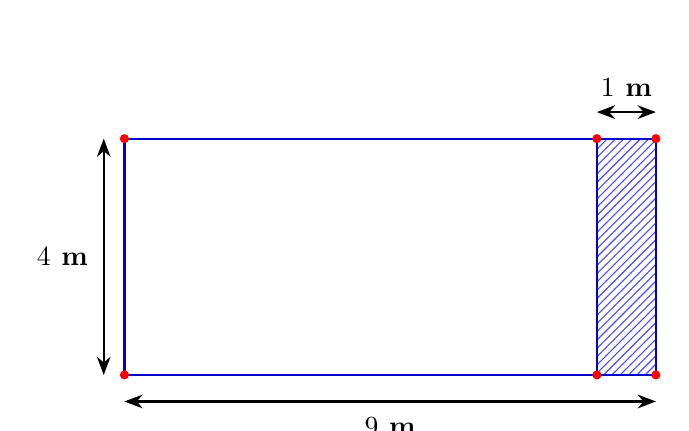
\begin{tikzpicture}[scale=0.75, line cap=round, line join=round, >=Stealth]
  \coordinate (A) at (0,4); \coordinate (B) at (9,4); \coordinate (C) at (9,0); \coordinate (D) at (0,0);
  \coordinate (E) at (8,4); \coordinate (F) at (8,0);
  \fill[pattern=north east lines, pattern color=blue!70] (E) rectangle (C);
  \draw[thick, blue!80!black] (D) rectangle (B);
  \draw[thick, blue!80!black] (E) -- (F);
  \foreach \p in {A,B,C,D,E,F} \fill[red] (\p) circle (2.2pt);
  \draw[<->, thick] (-0.35,0) -- (-0.35,4) node[midway, left=2pt, font=\bfseries] {$4\text{ m}$};
  \draw[<->, thick] (0,-0.45) -- (9,-0.45) node[midway, below=2pt, font=\bfseries] {$9\text{ m}$};
  \draw[<->, thick] (8,4.45) -- (9,4.45) node[midway, above=2pt, font=\bfseries] {$1\text{ m}$};
\end{tikzpicture}
\end{center}\
a) Tính diện tích phần sân dùng để trồng hoa.\
b) Nếu lát phần sân còn lại bằng những viên gạch hình vuông cạnh $40\text{ cm}$ thì cần bao nhiêu viên gạch? (Coi diện tích mạch ghép giữa các viên gạch là không đáng kể).
\end{enumerate}
\loigiai{
\begin{itemize}[leftmargin=0.5cm, itemsep=3pt]
\item \textbf{1)} Học sinh dùng thước thẳng và ê-ke vẽ đúng hình chữ nhật $ABCD$ có chiều dài $AB = CD = 5\text{ cm}$ và chiều rộng $BC = AD = 3\text{ cm}$:
\begin{center}
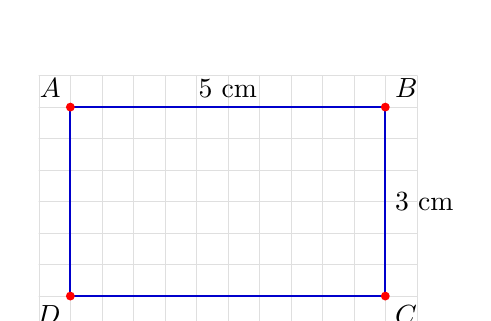
\begin{tikzpicture}[scale=0.8, line cap=round, line join=round]
  \draw[step=0.5cm, gray!25, very thin] (-0.5,-0.5) grid (5.5,3.5);
  \draw[thick, blue!80!black] (0,0) rectangle (5,3);
  \foreach \p/\pos in {(0,3)/above left, (5,3)/above right, (5,0)/below right, (0,0)/below left} {
    \fill[red] \p circle (2pt);
  }
  \node[above left] at (0,3) {$A$};
  \node[above right] at (5,3) {$B$};
  \node[below right] at (5,0) {$C$};
  \node[below left] at (0,0) {$D$};
  \node[above] at (2.5,3) {$5\text{ cm}$};
  \node[right] at (5,1.5) {$3\text{ cm}$};
\end{tikzpicture}
\end{center} \hfill \textbf{[0.25đ]}
\item \textbf{2)} a) Phần sân trồng hoa là hình chữ nhật có chiều rộng $1\text{ m}$ và chiều dài $4\text{ m}$.\
Diện tích phần sân trồng hoa là: $1 \times 4 = 4\text{ (m}^2\text{)}$.\
\
b) Diện tích của toàn bộ khoảng sân là: $9 \times 4 = 36\text{ (m}^2\text{)}$.\
Diện tích phần sân cần lát gạch là: $36 - 4 = 32\text{ (m}^2\text{)} = 320\,000\text{ (cm}^2\text{)}$.\
Diện tích của mỗi viên gạch hình vuông là: $40 \times 40 = 1600\text{ (cm}^2\text{)}$.\
Số viên gạch cần dùng để lát phần sân còn lại là: $320\,000 : 1600 = 200\text{ (viên)}$. \hfill \textbf{[0.5đ]}
\end{itemize}
}
\end{ex}
\vspace{1.5mm}

\begin{ex} (0.5 điểm)
\begin{enumerate}[label=\textbf{\alph*)}, leftmargin=0.8cm, itemsep=2pt]
\item Tính tổng $C = 1 + 3 + 3^2 + 3^3 + 3^4 + \dots + 3^{2020}$.
\item Tìm số tự nhiên $n$ sao cho $p = (n - 2)(n^2 + n - 5)$ là một số nguyên tố.
\end{enumerate}
\loigiai{
\begin{itemize}[leftmargin=0.5cm, itemsep=3pt]
\item \textbf{a)} Ta có: $C = 1 + 3 + 3^2 + 3^3 + 3^4 + \dots + 3^{2020}$.\
Nhân cả hai vế với 3:\
$3C = 3 + 3^2 + 3^3 + 3^4 + \dots + 3^{2021}$.\
Trừ vế với vế:\
$3C - C = (3 + 3^2 + \dots + 3^{2021}) - (1 + 3 + \dots + 3^{2020})$\
$\implies 2C = 3^{2021} - 1 \implies C = \dfrac{3^{2021} - 1}{2}$. \hfill \textbf{[0.25đ]}
\item \textbf{b)} Vì $p$ là số nguyên tố nên tích $p = (n - 2)(n^2 + n - 5)$ chỉ có hai ước tự nhiên là 1 và chính nó.\
Do đó một trong hai thừa số phải bằng 1 và thừa số còn lại phải là số nguyên tố.\
\
$\bullet$ Trường hợp 1: $n - 2 = 1 \implies n = 3$.\
Khi đó $p = 1 \cdot (3^2 + 3 - 5) = 1 \cdot (9 + 3 - 5) = 7$ (là số nguyên tố, thỏa mãn).\
\
$\bullet$ Trường hợp 2: $n^2 + n - 5 = 1 \implies n^2 + n - 6 = 0 \implies (n - 2)(n + 3) = 0$.\
Vì $n$ là số tự nhiên nên $n = 2$. Khi đó $n - 2 = 0 \implies p = 0$ (không phải số nguyên tố, loại).\
\
Vậy số tự nhiên cần tìm là $n = 3$. \hfill \textbf{[0.25đ]}
\end{itemize}
}
\end{ex}
\vspace{1.5mm}


\begin{center}
\rule{4cm}{0.4pt}\\
\textit{--- HẾT ---}
\end{center}
\end{document}
